\documentclass[11pt,a4paper]{report}

\usepackage[utf8]{inputenc}
\usepackage[portuges]{babel}
\usepackage{indentfirst}
\usepackage{graphicx}
\usepackage{float}
\usepackage{caption}
\usepackage{subcaption}
\usepackage[T1]{fontenc}
\usepackage{listings}
\usepackage{amsmath}
\usepackage{mathtools}
\usepackage{tikz}
\usepackage{qtree}
\usepackage{listings, xcolor}
\lstset{
tabsize = 4, %% Sets tab space width.
showstringspaces = false, %% Prevents space marking in strings, string is defined as the text that is generally printed directly to the console.
numbers = left, %% Displays line numbers on the left.
commentstyle = \color{green}, %% Sets comment color.
keywordstyle = \color{blue}, %% Sets  keyword color.
stringstyle = \color{red}, %% Sets  string color.
rulecolor = \color{black}, %% Sets frame color to avoid being affected by text color.
basicstyle = \small \ttfamily , %% Sets listing font and size.
breaklines = true, %% Enables line breaking.
numberstyle = \tiny,
}
\renewcommand{\familydefault}{\sfdefault}

% packages que adicionei do stor
\usepackage{xspace}
\setlength{\oddsidemargin}{-1cm}
\setlength{\textwidth}{18cm}
\setlength{\headsep}{-1cm}
\setlength{\textheight}{23cm}

\title{Processamento de Linguagens (3º ano de Curso)\\
	\textbf{Trabalho Prático Nº3 (YACC)}\\ Relatório de Desenvolvimento}
\author{Diogo Braga\\ A82547 \and João Silva\\ A82005 \and Ricardo Caçador\\ A81064}
\date{\today}

\begin{document}

\maketitle

\begin{abstract}
	Neste relatório é apresentada a resolução de um exercício referente ao TP3, que tem como principais objetivos:
	\begin{itemize}
		\item aumentar a experiência de uso do ambiente \textbf{Linux}, da linguagem imperativa  \textbf{C}, e de algumas ferramentas de apoio à programação;
 		\item rever e aumentar a capacidade de escrever \textit{gramáticas independentes de contexto (GIC)}, que satisfaçam a condição LR(), para criar Linguagens de Domínio Específico (DSL);
 		\item desenvolver processadores de linguagens segundo o método da \textit{tradução dirigida pela sintaxe}, suportado numa \textit{gramática tradutora (GT)};
 		\item utilizar geradores de compiladores como o par \textbf{flex/yacc}.
	\end{itemize}
\end{abstract}

\tableofcontents

\newpage

\chapter{Introdução}
\label{chap:intro}

Seguindo a fórmula \emph{exercício = (N\_Alu\% 6)  +  1} e o número de aluno mais alto presente no nosso grupo (82547), o enunciado correspondente é o \textbf{6  -  Construtor de diaporama}.

Este enunciado apresentou-nos um tipo de apresentações visuais suportadas por um conjunto de diapositivos ou acetatos/slides que é conhecido como \textbf{Diaporama}. O \textbf{diaporama} é uma sequência de elementos. Cada elemento pode ser/conter:
\begin{itemize}
	\item Uma página inicial de abertura e créditos;
	\item imagens;
	\item páginas simples (exemplo:  uma lista de items);
	\item video;
	\item opcionalmente, título;
	\item opcionalmente, audio.
\end{itemize}

Tendo estes aspetos em conta é requerido que se crie uma sequência de páginas HTML temporizadas, em que cada página HTML corresponderá a um diapositivo.

Com este relatório pretendemos apresentar as nossas opções e algoritmos desenvolvidos para a realização do gerador de diaporamas. Pretendemos também apoiar aquelas que foram as nossas soluções, com conhecimento obtido nas aulas teóricas.

Para uma melhor visão do que irá ser abordado neste relatório deixamos uma breve descrição daquilo que foi feito. No segundo capítulo foi feita uma análise informal e uma especificação dos requisitos deste projeto. No terceiro capítulo foi realizado o desenho da conceção no qual estão envolvidos os algoritmos e estruturas de dados usados. No quarto capítulo mostramos alguns exemplos de implementações e vários resultados de testes realizados. No quinto capítulo apresentamos as funcionalidades estendidas do nosso projeto. Por último no capítulo 6 fazemos uma retrospetiva do trabalho realizado e concluímos.


\chapter{Análise e Especificação}
\label{chap:analise}

Analisando o problema como um todo, a fase de análise foi bastante simples e curta. Bastou apenas seguir o enunciado para começar a pensar o que seria um \textbf{diaporama}, que elementos poderia conter, que tipo de slides poderia apresentar bem como a disposição do conteúdo a apresentar.

No final desta supervisão do conceito de \textbf{diaporama} apuramos todos os elementos que este poderia conter, que são nomeadamente:

\begin{itemize}
	\item Um nome da apresentação;
	\item Diapositivos, cada um contendo:
	\begin{itemize}
		\item Tempo de disposição;
		\item Body, onde reside conteúdo, que pode ser/conter de diversos tipos, nomeadamente:
		\begin{itemize}
			\item Uma página inicial de abertura e créditos;
			\item Imagens;
			\item Páginas simples (exemplo:  uma lista de items);
			\item Vídeo;
			\item Título;
			\item Áudio.
		\end{itemize}
	\end{itemize}
\end{itemize}

De referir ainda que cada tipo de diapositivos é aprofundado contendo variados parâmetros que serão apresentados no próximo capítulo.

Por último, após a análise dum diaporama, foi de grande relevância a investigação por conteúdo \textbf{HTML} que pudesse representar numa página cada tipo de diapositivo anteriormente definido.

\chapter{Conceção/desenho da Resolução}
\label{chap:concecao}

Neste capítulo baseamo-nos nas análises anteriormente efetuadas que serviram de base inicial para a construção duma \textbf{gramática independente de contexto (GIC)} que representasse um diaporama e consequentemente para a construção duma \textbf{gramática tradutora (GT)} que despontasse determinadas ações consoante o momento de parsing em que se encontrava.

Foi também necessário construir um \textbf{Analisador Léxico} que apoiasse a o reconhecimento e conversão de símbolos terminais da gramática.


\section{Gramática Independente de Contexto}

Tendo em conta a análise realizada construímos uma \textit{Gramática Independente de Contexto} \textbf{G = (T, NT , S, P)}, em que \textbf{T} é conjunto de terminais, \textbf{NT} é o conjunto de não terminais, \textbf{S} é o axioma e \textbf{P} é o conjunto de produções. A gramática \textbf{G} pode então ser definida por:

\vspace{0.5cm}

\textbf{T} = \{ STYLE, DIAPOSITIVO, CRED, IMG, LI, VID, LB, TITL, AUD, ',' , ';' , '\{' , '\}' , '(' , ')' , NUM, STRING\}

\vspace{0.5cm}

\textbf{NT} = \{ Diaporama, Nome, Estilo, Elementos, Elemento, Body, Tipos, Tipo, Credito, Imagem, Item, Video, LineBreak, Opcoes, Titulo, Audio, Tempo, Width, Height \}

\vspace{0.5cm}

\textbf{S} = \{ Diaporama \}

\vspace{0.5cm}

\textbf{P} = \{ Diaporama $\rightarrow$ Nome ',' Elementos

\vspace{0.2cm}
\hspace{3.15cm} | Nome ',' STYLE Estilo ',' Elementos

\vspace{0.2cm}
\hspace{1.0cm} Nome $\rightarrow$ STRING

\vspace{0.2cm}
\hspace{1.0cm} Estilo $\rightarrow$ STRING

\vspace{0.2cm}
\hspace{1.0cm} Elementos $\rightarrow$ Elemento

\vspace{0.2cm}
\hspace{3.05cm} | Elementos ',' Elemento

\vspace{0.2cm}
\hspace{1.0cm} Elemento $\rightarrow$ DIAPOSITIVO '\{' Tempo ';' Body '\}'

\vspace{0.2cm}
\hspace{1.0cm} Tempo $\rightarrow$ NUM

\vspace{0.2cm}
\hspace{1.0cm} Body $\rightarrow$ '(' Opcoes ')' ',' Tipos

\vspace{0.2cm}
\hspace{2.3cm} | Tipos

\vspace{0.2cm}
\hspace{1.0cm} Tipos $\rightarrow$ Tipo

\vspace{0.2cm}
\hspace{2.3cm} | Tipos ',' Tipo

\vspace{0.2cm}
\hspace{1.0cm} Tipo $\rightarrow$ Credito

\vspace{0.2cm}
\hspace{2.2cm} | Imagem

\vspace{0.2cm}
\hspace{2.2cm} | Item

\vspace{0.2cm}
\hspace{2.2cm} | Video

\vspace{0.2cm}
\hspace{2.2cm} | LineBreak

\vspace{0.2cm}
\hspace{1.0cm} Credito $\rightarrow$ CRED STRING

\vspace{0.2cm}
\hspace{1.0cm} Imagem $\rightarrow$ IMG STRING

\vspace{0.2cm}
\hspace{2.65cm} | IMG STRING Width Height

\vspace{0.2cm}
\hspace{1.0cm} Width $\rightarrow$ NUM

\vspace{0.2cm}
\hspace{1.0cm} Height $\rightarrow$ NUM

\vspace{0.2cm}
\hspace{1.0cm} Item $\rightarrow$ LI STRING

\vspace{0.2cm}
\hspace{1.0cm} Video $\rightarrow$ VID STRING

\vspace{0.2cm}
\hspace{2.3cm} | VID STRING Width Height

\vspace{0.2cm}
\hspace{1.0cm} LineBreak $\rightarrow$ LB

\vspace{0.2cm}
\hspace{1.0cm} Opcoes $\rightarrow$ Opcoes ',' Audio

\vspace{0.2cm}
\hspace{2.6cm} | Opcoes ',' Titulo

\vspace{0.2cm}
\hspace{2.6cm} | Titulo

\vspace{0.2cm}
\hspace{2.6cm} | Audio

\vspace{0.2cm}
\hspace{1.0cm} Titulo $\rightarrow$ TITL STRING

\vspace{0.2cm}
\hspace{1.0cm} Audio $\rightarrow$ AUD STRING


\hspace{0.7cm} \}

\vspace{0.5cm}

Tendo em conta que estamos perante a ferramenta \textbf{YACC} temos que considerar que o parsing da gramática é feito \textbf{Bottom-Up} segundo um algoritmo \textbf{LR} pelo que não podem existir conflitos.

Construindo o autómato \textbf{LR} para esta gramática é possível verificar que nem o conflito \textbf{Shift-Reduce}, nem o conflito \textbf{Reduce-Reduce} acontecem pelo que a gramática está pronta para ser usada.


\section{Analisador Léxico}

Foi construído um analisador léxico que apoiasse a o reconhecimento e conversão de símbolos terminais da gramática, escrito em \textbf{Flex}.

Este analisador tem duas principais funções:

\begin{itemize}
	\item \textit{Reconhecimento:} identificação de sequências de caracteres que são instâncias de classes de símbolos terminais;
	\item \textit{Conversão:} obtenção da representação mais conveniente do símbolo reconhecido.
\end{itemize}

O analisador desenvolvido encontra-se a seguir:

\vspace{0.5cm}

\begin{lstlisting}[language = Tex , frame = trBL , firstnumber = 1 , escapeinside={(*@}{@*)}]
%%
STYLE                               {return STYLE;}
DIAPOSITIVO                         {return DIAPOSITIVO;}
CRED                                {return CRED;}
IMG                                 {return IMG;}
LI                                  {return LI;}
VID                                 {return VID;}
LB                                  {return LB;}
TITL                                {return TITL;}
AUD                                 {return AUD;}
[,;{}()]                            {return yytext[0];}
[0-9]+                              {yylval.num = atof(yytext); return NUM;}
\"[^\"]*\"                          {char* str = removeTokens(yytext);
				      				 yylval.str = strdup(str); return STRING;}
.|\n                                {;}
%%

int yywrap() {return 1;}

char* removeTokens(char* s){
    char *p = s;
    p++;
    p[strlen(p)-1] = 0;
    return p;
}
\end{lstlisting}

\vspace{0.5cm}

De referir uma pequena particularidade no que toca ao reconhecimento de \textbf{Strings}. Estas têm que vir delimitadas por \textbf{""} uma vez que esta é a forma de saber quando começar a reconhecer e quando parar de filtrar. Após o reconhecimento baseado no requisito aqui colocado esta delimitação é retirada pela função \textbf{removeTokens(char* s)} definida no ficheiro.

Desta forma conseguimos reconhecer e converter todos os símbolos necessários para o parsing da gramática.



\section{Gramática Tradutora}

No reconhecimento de linguagens, tanto regulares como não-regulares, é necessário executar ações semâticas ao longo do reconhecimento sintático. Devido ao enunciado proposto, as ações semânticas apresentadas consistem em ações de tradução de frases reconhecidas em novas frases de outra linguagem, neste caso, HTML.

O processo de extensão da gramática independente de contexto com ações semânticas para obtenção duma gramática tradutora é apresentado nesta secção.

Antes da GIC, importante referir a existência das seguintes variáveis definidas:

\begin{itemize}
	\item \hspace{0.5cm} char* pasta; $\rightarrow$ Caminho para a pasta que contem os diapositivos criados;
	\item \hspace{0.5cm} int slide\_counter = 0; $\rightarrow$ Contador que possui o número do slide em tradução;
	\item \hspace{0.5cm} int tempo = 0; $\rightarrow$ Contador que possui o tempo da apresentação;
	\item \hspace{0.5cm} int imagens = 0; $\rightarrow$ Contador que possui o número de imagens da apresentação;
	\item \hspace{0.5cm} int videos = 0; $\rightarrow$ Contador que possui o número de vídeos da apresentação;
	\item \hspace{0.5cm} int audios = 0; $\rightarrow$ Contador que possui o número de áudios da apresentação;
	\item \hspace{0.5cm} FILE *file; $\rightarrow$ Ficheiro para o qual as traduções em HTML são escritas;
	\item \hspace{0.5cm} char* style\_file; $\rightarrow$ Caminho para a pasta que contem os ficheiros CSS;
	\item \hspace{0.5cm} int style = 0; $\rightarrow$ Flag que verifica se existem ficheiros CSS;
\end{itemize}


Para cada símbolo não-terminal, são de seguida exibidas as explicações das ações semânticas relacionadas:

\begin{itemize}
	\item Diaporama
	\begin{itemize}
		\item \underline{Nome ',' Elementos}  $\rightarrow$ Inserção do último diaporama, que contêm estatísticas, no ficheiro em utilização, com recurso à linguagem HTML (tag \textbf{html});
		\item \underline{Nome ',' STYLE Estilo ',' Elementos}  $\rightarrow$ Inserção do último diaporama, que contêm estatísticas, no ficheiro em utilização, com recurso à linguagem HTML e ao ficheiro CSS estabelecido (tag \textbf{html}, tag \textbf{link} e tag \textbf{body});
	\end{itemize}
	\item Nome
	\begin{itemize}
		\item \underline{STRING}  $\rightarrow$ Definição do noma pasta a ser criada, e consequente criação da mesma;
	\end{itemize}
	\item Estilo
	\begin{itemize}
		\item \underline{STRING}  $\rightarrow$ Atribuição do ficheiro CSS à variável style\_file, e ativação da flag style;
	\end{itemize}
	\item Elementos
	\item Elemento
	\begin{itemize}
		\item \underline{DIAPOSITIVO '{' Tempo ';' Body '}'}  $\rightarrow$ Inserção das tags que marcam o final do ficheiro em utilização, em linguagem HTML (tag \textbf{body} e tag \textbf{html});
	\end{itemize}
	\item Body
	\item Tipos
	\item Tipo
	\item Credito
	\begin{itemize}
		\item \underline{CRED STRING} $\rightarrow$ Inserção dum crédito no ficheiro em utilização, com recurso à linguagem HTML (tag \textbf{p});
	\end{itemize}
	\item Imagem
	\begin{itemize}
		\item \underline{IMG STRING}  $\rightarrow$ Inserção duma imagem no ficheiro em utilização, com recurso à linguagem HTML (tag \textbf{img}); Incremento do contador de imagens;
		\item \underline{IMG STRING Width Height}  $\rightarrow$ Inserção duma imagem com medidas estabelecidas no ficheiro em utilização, com recurso à linguagem HTML (tag \textbf{img}); Incremento do contador de imagens;
	\end{itemize}
	\item Item
	\begin{itemize}
		\item \underline{LI STRING}  $\rightarrow$ Inserção dum item no ficheiro em utilização, com recurso à linguagem HTML (tag \textbf{LI});
	\end{itemize}
	\item Video
	\begin{itemize}
		\item \underline{VID STRING}  $\rightarrow$ Inserção dum vídeo no ficheiro em utilização, com recurso à linguagem HTML (tag \textbf{iframe}); Incremento do contador de vídeos;
		\item \underline{VID STRING Width Height}  $\rightarrow$ Inserção dum vídeo com medidas estabelecidas no ficheiro em utilização, com recurso à linguagem HTML (tag \textbf{iframe}); Incremento do contador de vídeos;
	\end{itemize}
	\item LineBreak
	\begin{itemize}
		\item \underline{LB}  $\rightarrow$ Inserção duma quebra de linha no ficheiro em utilização, com recurso à linguagem HTML (tag \textbf{br});
	\end{itemize}
	\item Opcoes
	\item Titulo
	\begin{itemize}
		\item \underline{TITL STRING}  $\rightarrow$ Inserção dum título no ficheiro em utilização, com recurso à linguagem HTML (tag \textbf{h1});
	\end{itemize}
	\item Audio
	\begin{itemize}
		\item \underline{AUD STRING}  $\rightarrow$ Inserção dum áudio no ficheiro em utilização, com recurso à linguagem HTML (tag \textbf{audio}); Incremento do contador de áudios;
	\end{itemize}
	\item Tempo
	\begin{itemize}
		\item \underline{NUM}  $\rightarrow$ Aumento do contador do número do slide em tradução; Aumento do tempo da apresentação; Criação dum ficheiro "diapX.html" que vai ser utilizado na tradução e introdução do mesmo na pasta estabelecida; Decisão da utilização do ficheiro CSS consoante a flag style, e consequente inserção do cabeçalho no ficheiro em utilização, com recurso à linguagem HTML (tag \textbf{html}, tag \textbf{head}, tag \textbf{link}, tag \textbf{meta} e tag \textbf{body});
	\end{itemize}
	\item Width
	\item Height
\end{itemize}

\newpage

\subsection{Funções em C}

Uma vez que foi necessário criar ficheiros \textbf{HTML} e consequentemente criar pastas onde residem estes ficheiros, foi necessário o auxílio de funções escritas em \textbf{C} para completar esta tarefa e para que o código presente no ficheiro onde reside a gramática não se tornasse muito extenso.

Deste modo na sequência desta ideia apresentamos abaixo as funções requeridas, que estão declaradas no ficheiro \textbf{auxiliares.h} e definidas no ficheiro \textbf{auxiliares.c}.

\vspace{0.5cm}

\begin{lstlisting}[language = C , frame = trBL , firstnumber = 1 , escapeinside={(*@}{@*)}]
FILE* createFile(int num, char* pasta);

void makeheader(int tempo, FILE* file, int num);

void makeheaderStyle(int tempo, FILE* file, int num, char* style_file);

void insertTitle(FILE* file, char* title);

void insertAudio(FILE* file, char* audio);

void insertItem(FILE* file, char* item);

void insertImage(FILE* file, char* image);

void insertImageSize(FILE* file, char* image, int width, int height);

void insertVideo(FILE* file, char* video);

void insertVideoSize(FILE* file, char* video, int width, int height);

void insertLineBreak(FILE* file);

void fileTermination(FILE* file);

void createLastFile(int num, char* pasta);

void createLastFileStyle(int num, char* pasta, char* style_file);

\end{lstlisting}

\chapter{Codificação e Testes}
\label{chap:codificacao}

Para a presente secção foram extremamente importantes as duas secções anteriores. Desta forma apresentamos alternativas, decisões, problemas de implementação, testes realizados e ainda exemplos de inputs para a gramática construída.


\section{Alternativas, Decisões e Problemas de Implementação}

Nesta secção é importante falar das decisões que são necessárias ser tomadas por exemplo nas imagens, nos vídeos, ou ainda no momento de escolher ou não um estilo associado ao ficheiro HTML.

No caso das imagens, tal acontece porque estas possuem um tamanho, e por predefinição é esse o tamanho apresentado no diaporama. No entanto, este pode ser alterado, e desta forma é necessário decidir qual das vias é tomada, passando os dois parâmetros para a altura e a largura, ou então não o fazendo e ficando a imagem com o tamanho predefinido. Nos vídeos sucede-se a mesma decisão.

Quanto ao caso de inclusão ou não do ficheiro CSS, tal é realizado no momento da criação do \textit{head} do ficheiro HTML. Caso a variável \textbf{style} esteja positiva o estilo é usado, e caso contrário o ficheiro HTML não é associado a nenhum estilo CSS.

\section{Estruturas dos Inputs}

Olhando para a gramática construída anteriormente é preciso construir um input para que esta o consuma e crie um output. Um exemplo de \textbf{Input} é o que se encontra a seguir:

\begin{figure}[H]
\centering
\frame{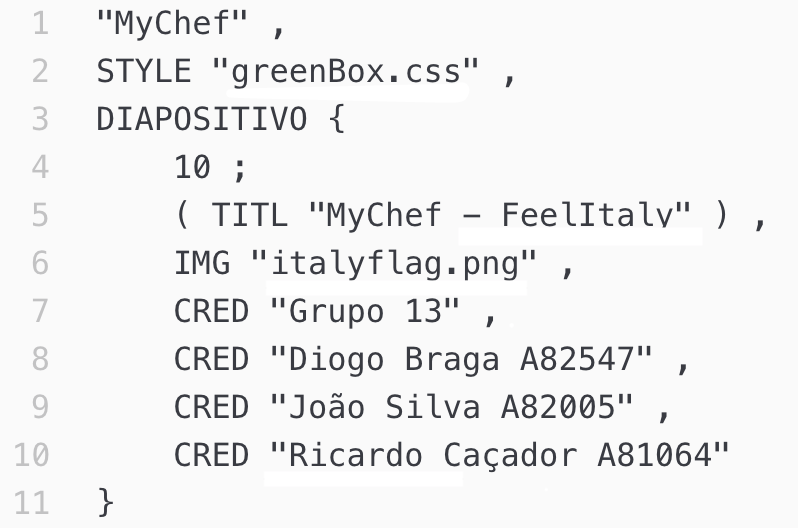
\includegraphics[scale=0.6]{input.png}}
\caption{Estrutura dum Input possível}
\label{img:input}
\end{figure}

A prova de que o input acima é aceite pela gramática encontra-se a seguir com a seguinte árvore de derivação:

% http://ironcreek.net/phpsyntaxtree/?
%[Diaporama [Nome [STRING "MyChef"]][','] [STYLE] [Estilo [STRING "greenBox.css"]] [','] [Elementos [Elemento [DIAPOSITIVO] ['{'] [Tempo [NUM 10]] [';'] [Body ['('] [Opcoes [Titulo [TITL] [STRING "MyChef - FeelItaly"]]] [')'] [','] [Tipos [Tipos [Tipos [Tipos [Tipos [Tipo [Imagem [IMG] [STRING "italyflag.png"]]]] [','] [Tipo [Credito [CRED] [STRING "Grupo 13"]]]] [','] [Tipo [Credito [CRED] [STRING "Diogo Braga A82547"]]]] [','] [Tipo [Credito [CRED] [STRING "João Silva A82005"]]]] [','] [Tipo [Credito [CRED][STRING "Ricardo Caçador A81064"]]]]] ['}'] ]]]

\begin{figure}[H]
\centering
\noindent
\makebox[\textwidth]{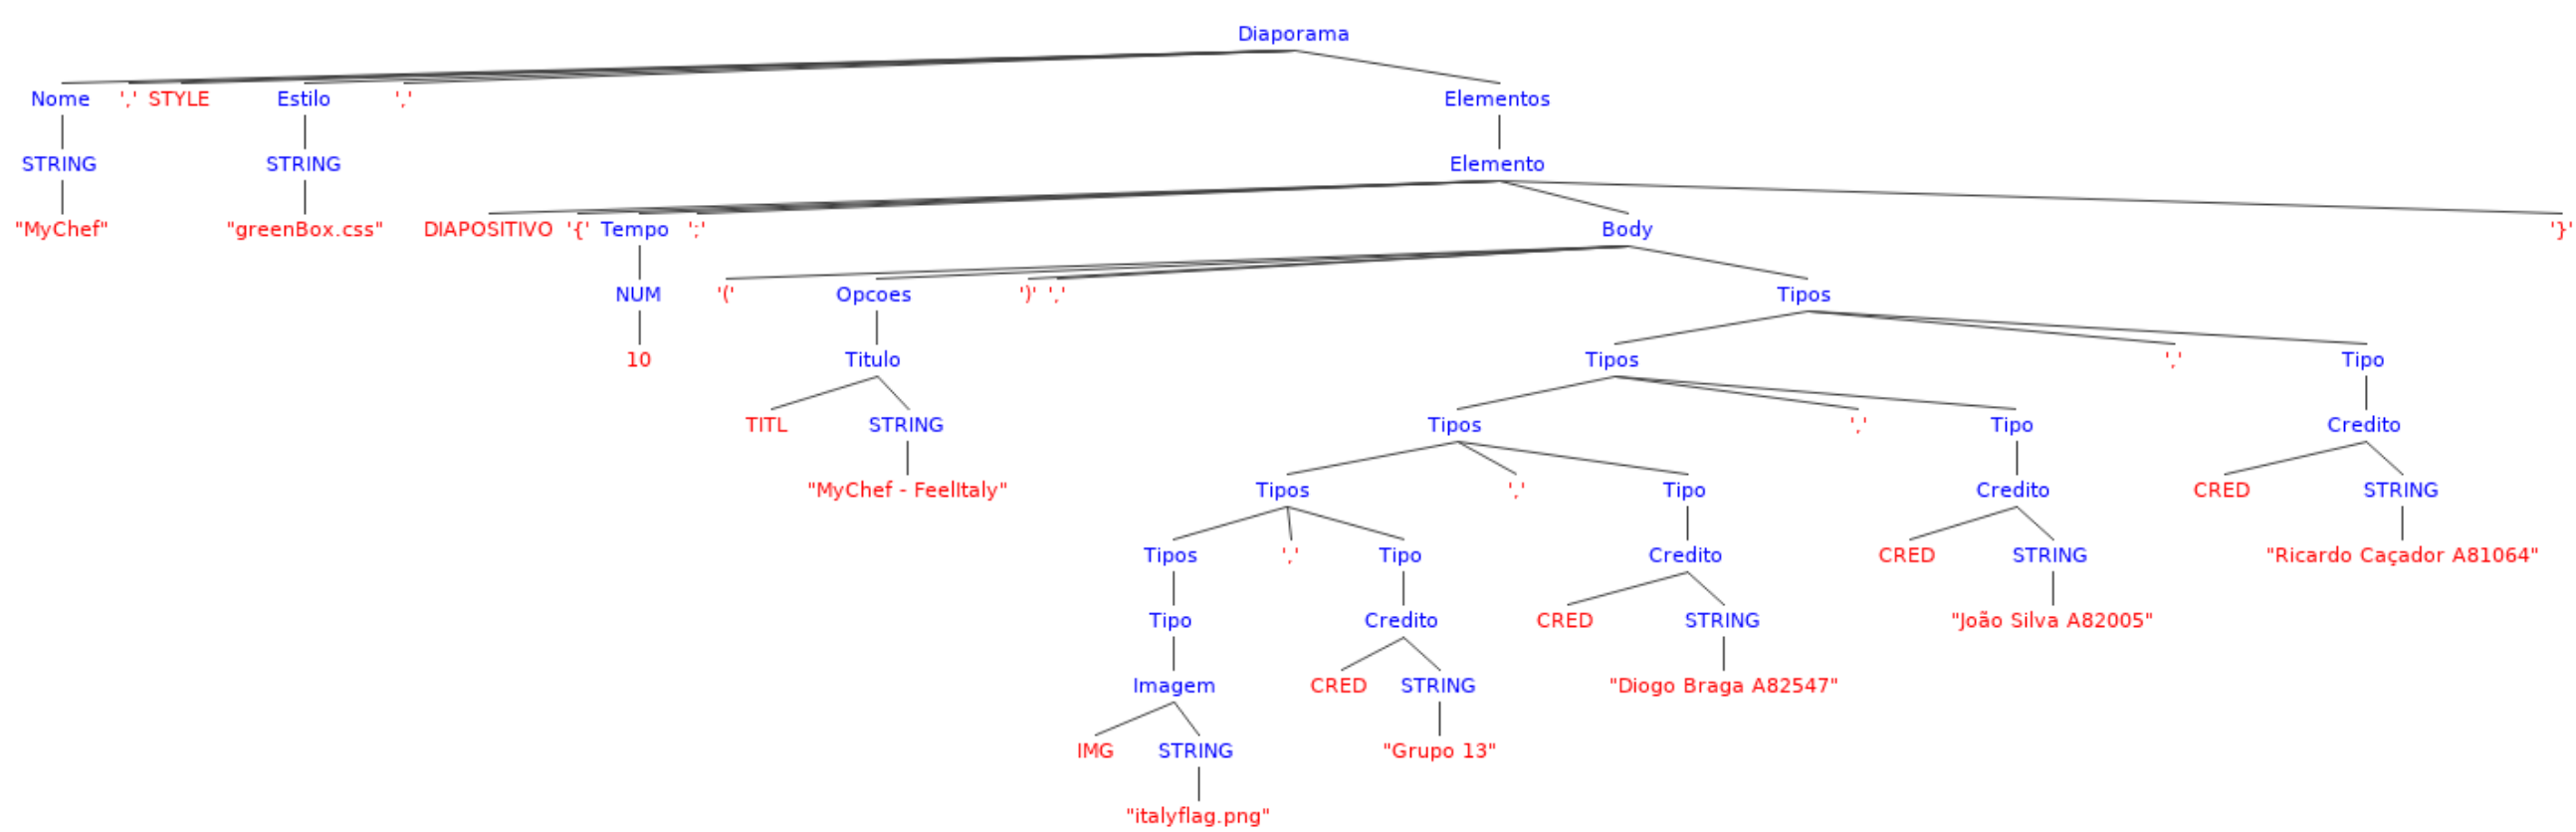
\includegraphics[width=19cm,height=13cm]{arvoreDerivacao.png}}
\caption{Árvore de Derivação duma frase}
\label{img:derivacao}
\end{figure}

Considerando a frase apresentada na figura \ref{img:input}, e após realizar a derivação através da árvore de derivação apresentada na figura \ref{img:derivacao} dá para reparar que as folhas da árvore (pintadas a vermelho) corresponde exatamente à frase apresentada mais acima.

Desta forma a frase pertence à gramática definida.

\newpage

\section{Testes realizados e Resultados}

\subsection{Compilação e Invocação}

Uma vez que criamos uma makefile, o processo de compilação é muito simples e a forma de invocação também o é, contudo um exemplo de como correr o programa é apresentado a seguir:

\begin{lstlisting}[language = Bash , frame = trBL , firstnumber = 1 , escapeinside={(*@}{@*)}]
> make
>
> ./diap < inputMyChef
\end{lstlisting}


\subsection{Resultados}

Nesta secção são apresentados alguns resultados alcançados com a implementação criada, como por exemplo, títulos, imagens, créditos, itens, áudios, imagens e vídeos.

\begin{figure}[H]
\centering
\frame{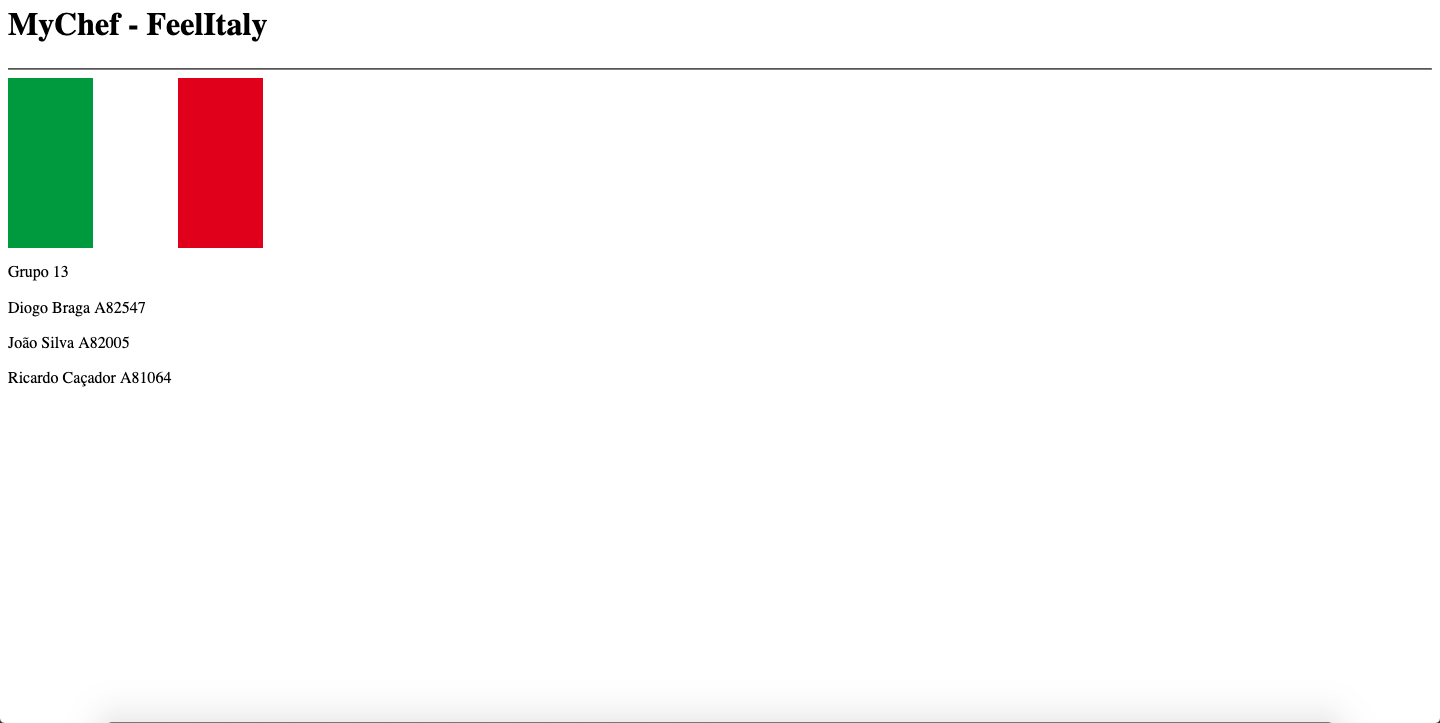
\includegraphics[scale=0.35]{exemplo1.png}}
\caption{Diaporama com um título, uma imagem e quatro créditos}
\label{img:exemplo1}
\end{figure}

\begin{figure}[H]
\centering
\frame{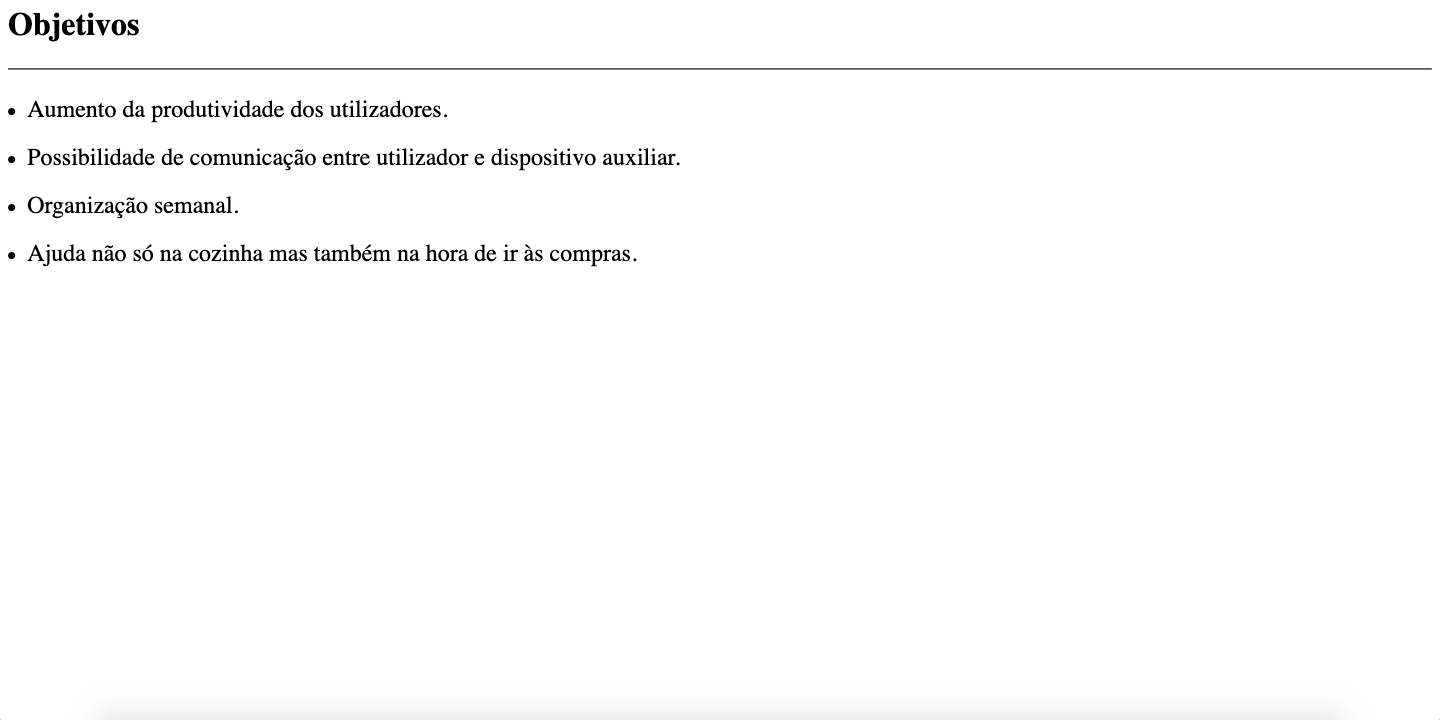
\includegraphics[scale=0.35]{exemplo3.png}}
\caption{Diaporama com um título e quatro itens}
\label{img:exemplo3}
\end{figure}

\begin{figure}[H]
\centering
\frame{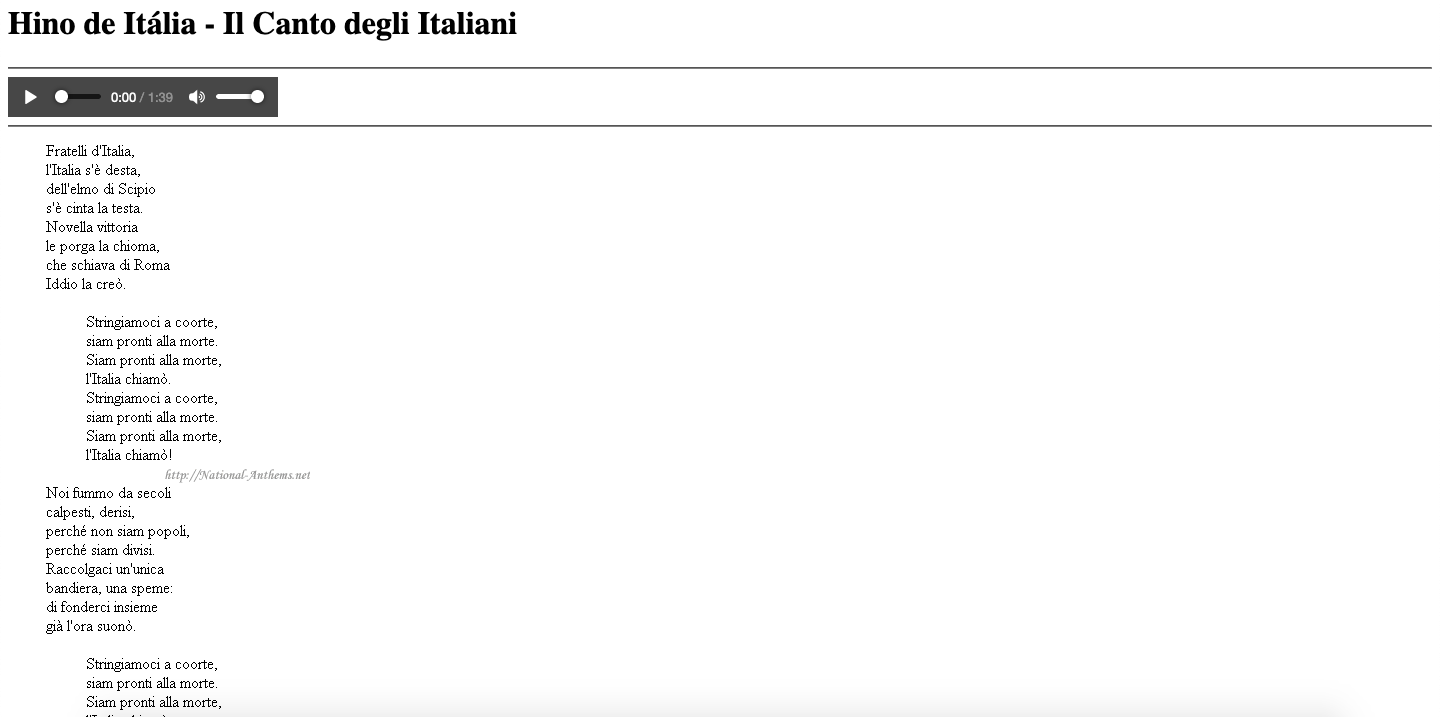
\includegraphics[scale=0.35]{exemplo5.png}}
\caption{Diaporama com um título, um áudio e uma imagem (fundo transparente)}
\label{img:exemplo5}
\end{figure}

\begin{figure}[H]
\centering
\frame{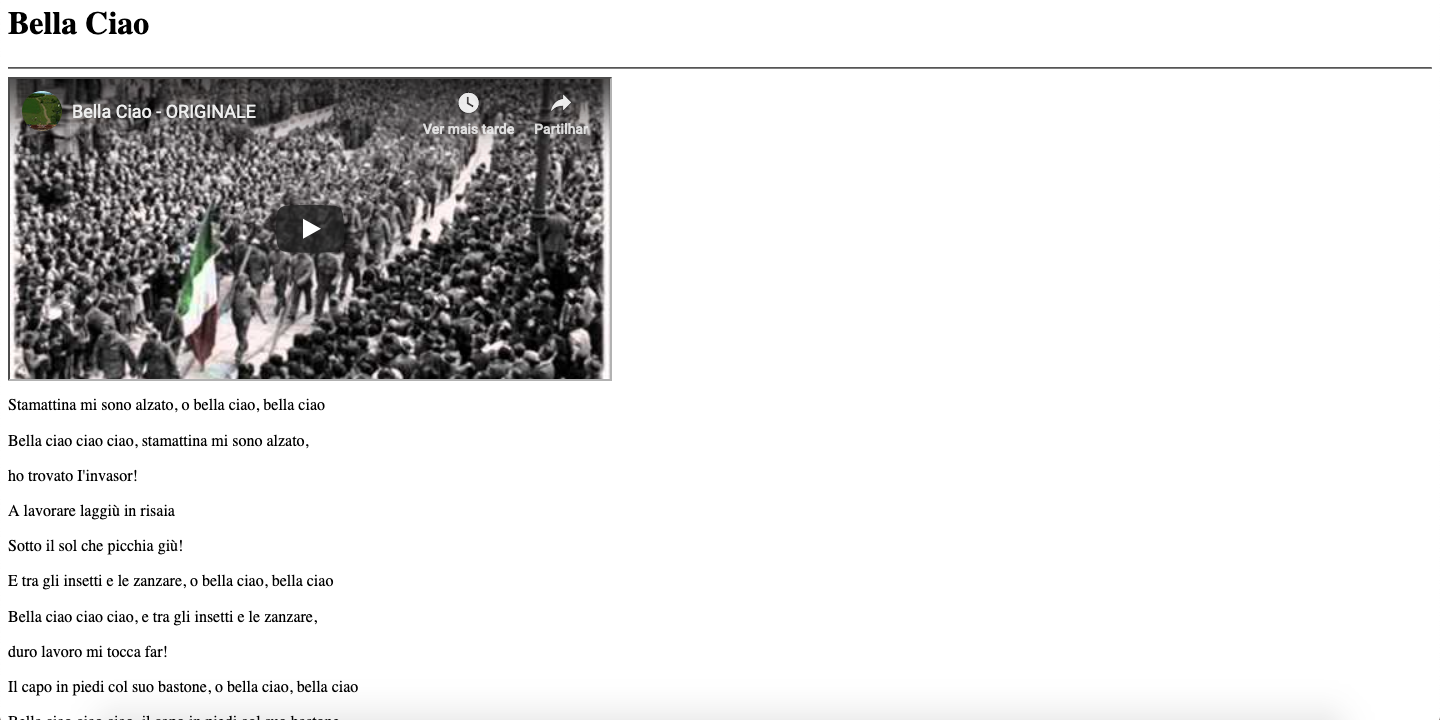
\includegraphics[scale=0.35]{exemplo7.png}}
\caption{Diaporama com um título, um vídeo e uma coleção de créditos}
\label{img:exemplo7}
\end{figure}


\chapter{Extras}
\label{chap:extras}

De forma a tornar os diaporamas mais organizados e apresentáveis, foi desenvolvido um ficheiro CSS para auxiliar o ficheiro HTML criado durante a execução das ações semânticas da gramática tradutora.

O ficheiro CSS realiza alterações ao nível das margens, do alinhamento e das cores, tanto ao nível do \textit{background} como das bordas.

Como foi criado um CSS para este efeito podem ser criados muitos mais e usá-los como estilo no diaporama a produzir, se bem que o CSS tem que se limitar a um conjunto reduzido de parâmetros que podem ser alterados.

Além do ficheiro CSS, foi também criado um diaporama final que é gerado automaticamente com estatísticas relacionadas com os diversos diaporamas presentes no ficheiro de input.

Por último, foi criada uma makefile de forma a facilitar a geração do executável em causa.

Os resultados são apresentados nas imagens seguintes.

\begin{figure}[H]
\centering
\frame{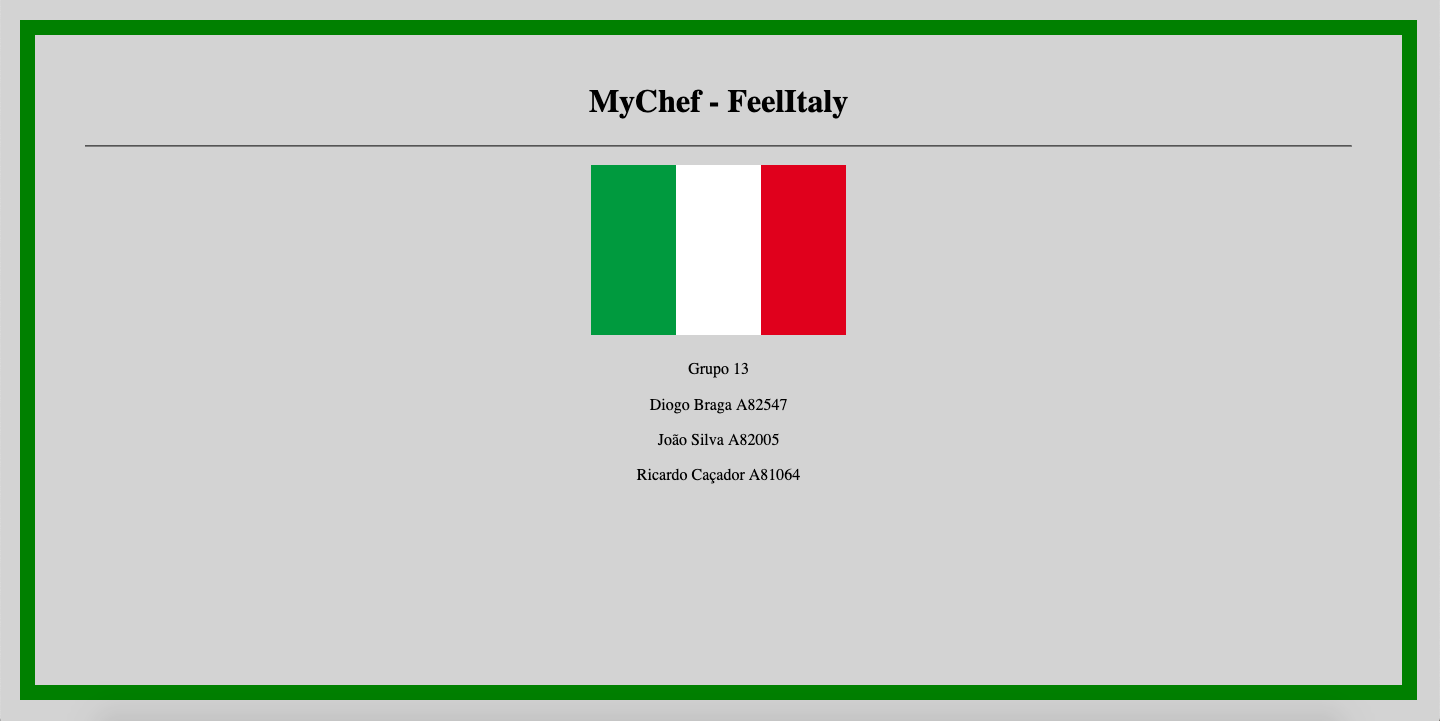
\includegraphics[scale=0.35]{exemplo2.png}}
\caption{Figura \ref{img:exemplo1} com estilo associado}
\label{img:exemplo2}
\end{figure}

\begin{figure}[H]
\centering
\frame{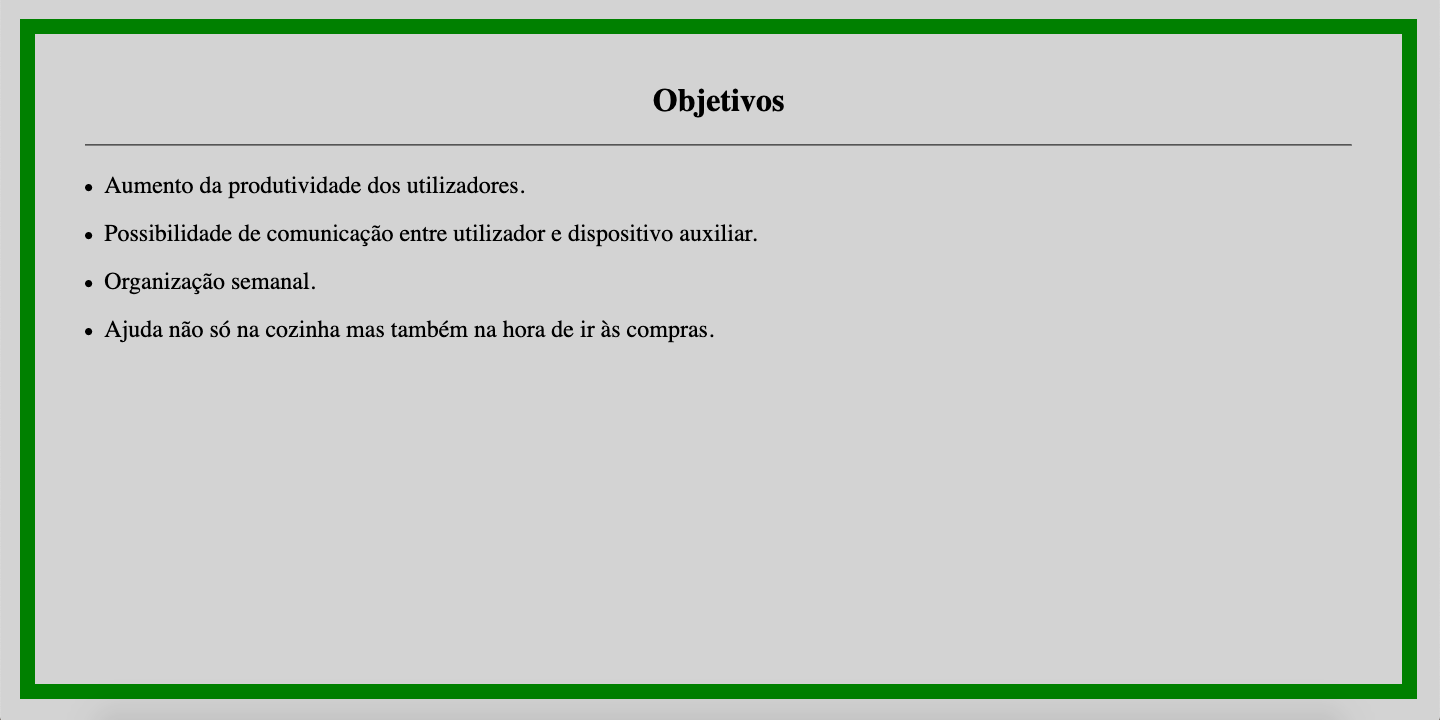
\includegraphics[scale=0.35]{exemplo4.png}}
\caption{Figura \ref{img:exemplo3} com estilo associado}
\label{img:exemplo4}
\end{figure}

\begin{figure}[H]
\centering
\frame{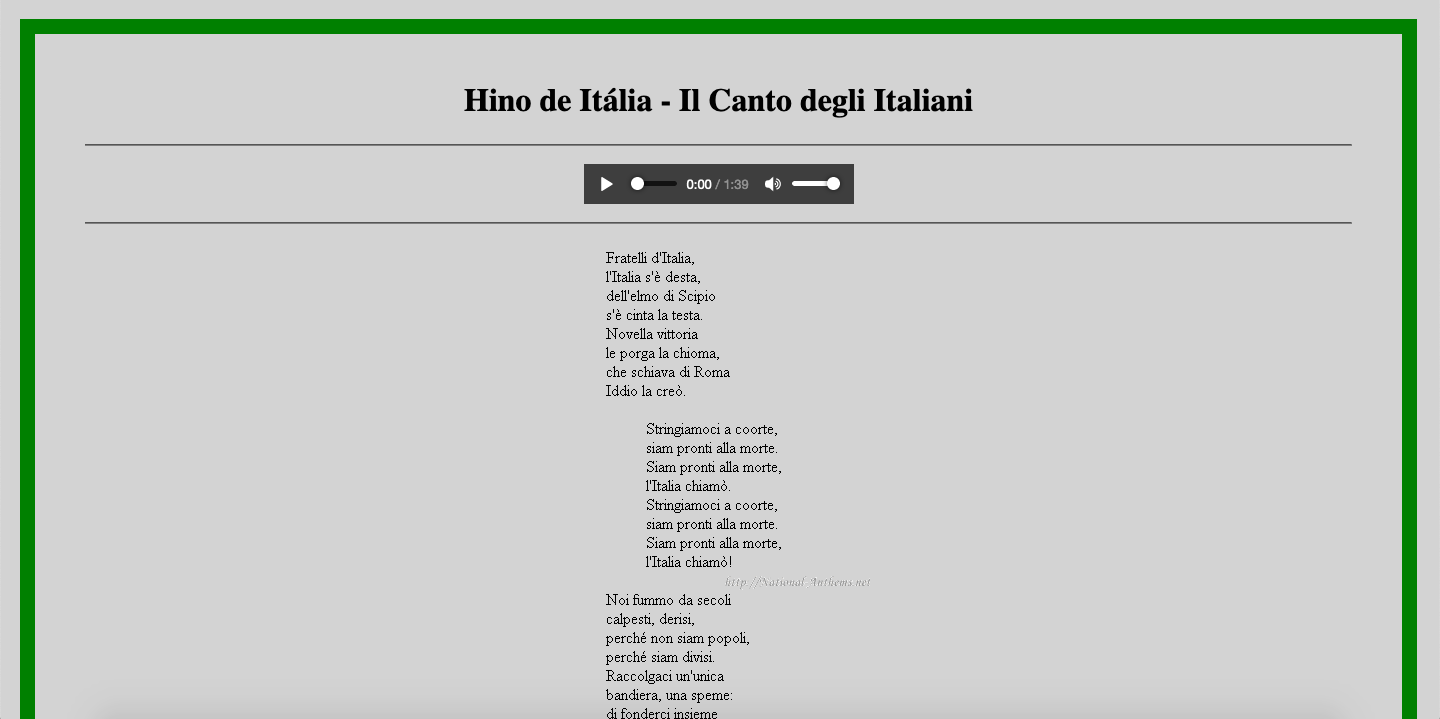
\includegraphics[scale=0.35]{exemplo6.png}}
\caption{Figura \ref{img:exemplo5} com estilo associado}
\label{img:exemplo6}
\end{figure}

\begin{figure}[H]
\centering
\frame{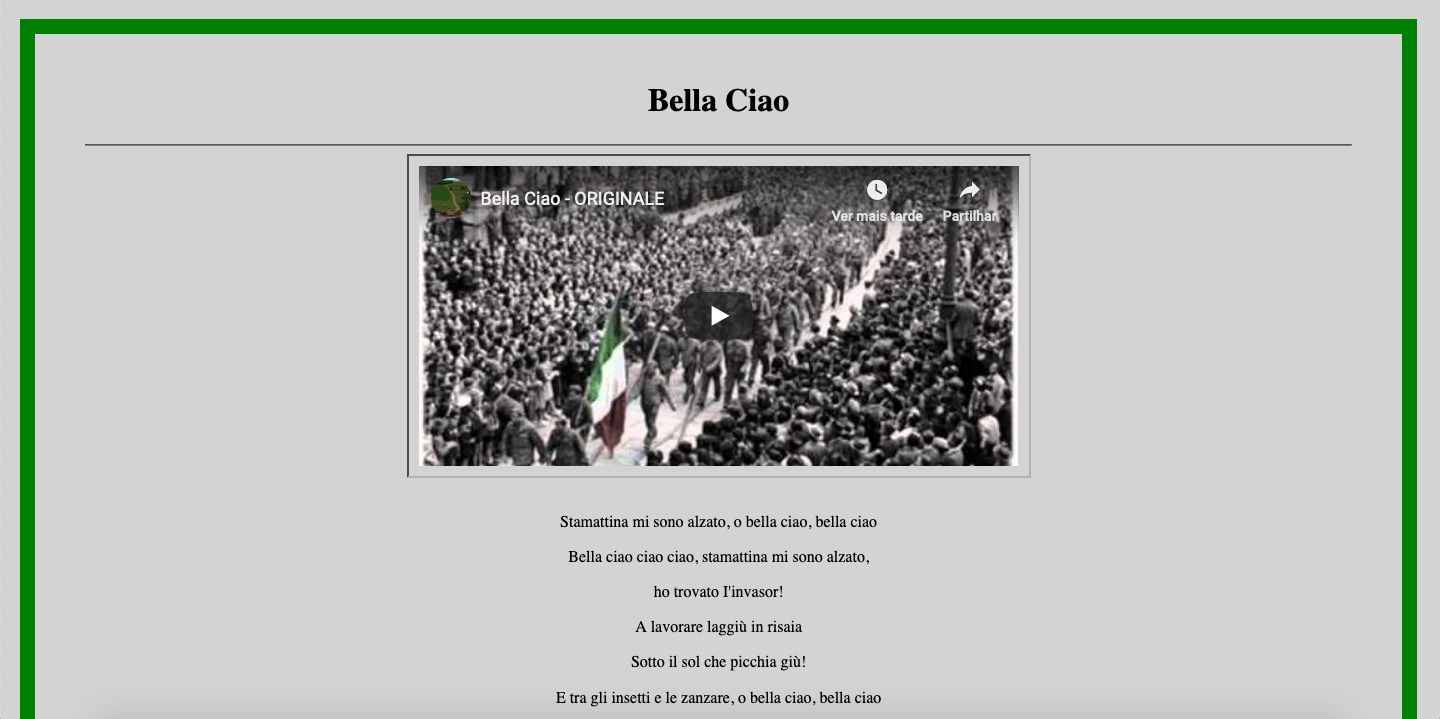
\includegraphics[scale=0.35]{exemplo8.png}}
\caption{Figura \ref{img:exemplo7} com estilo associado}
\label{img:exemplo8}
\end{figure}

\begin{figure}[H]
\centering
\frame{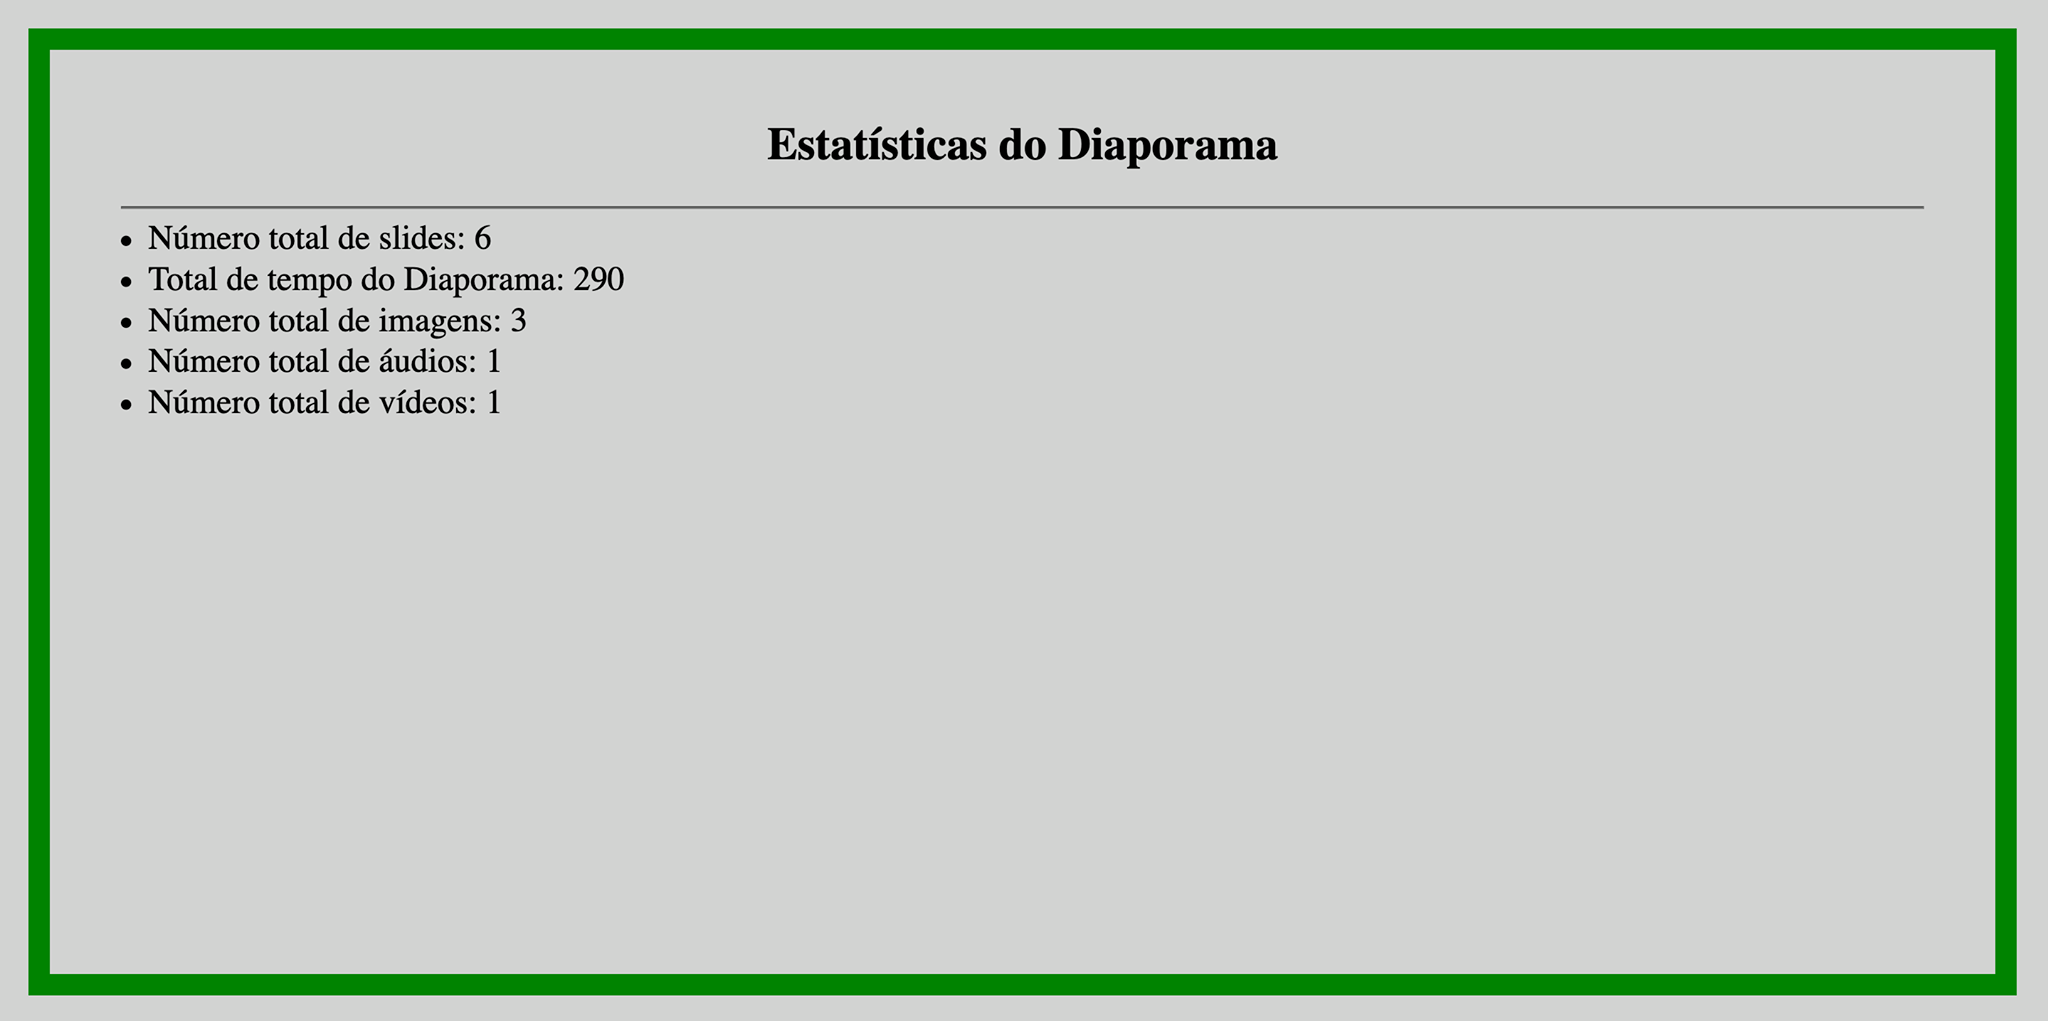
\includegraphics[scale=0.25]{exemplo9.png}}
\caption{Diaporama com estatísticas}
\label{img:exemplo9}
\end{figure}

\chapter{Conclusão}
\label{chap:concl}

Tendo em conta os requisitos deste projeto, e o trabalho realizado pelo grupo, achamos que os objetivos fundamentais foram atingidos, sendo estes rever e aumentar a capacidade de escrever \textit{gramáticas independentes de contexto (GIC)}, que satisfaçam a condição LR(), para criar Linguagens de Domínio Específico (DSL), desenvolver processadores de linguagens segundo o método da \textit{tradução dirigida pela sintaxe}, suportado numa \textit{gramática tradutora (GT)} e por último utilizar geradores de compiladores como o par \textbf{flex/yacc}.

Ao longo da realização deste projeto o grupo procurou incluir vários parâmetros na gramática de forma a completá-la sempre mais e a chegar à melhor resolução possível. É exemplo disso a inclusão de estilos (CSS) para produzir um resultado que fosse o mais idêntico a uma disposição de slides.

O grupo tentou também apurar ao máximo o espírito crítico, de forma a tomar as melhores decisões nos algoritmos tendo em conta as capacidades das ferramentas usadas, sendo que este foi também um dos maiores desafios encontrados.

Em jeito de conclusão o grupo acha que o problema requisitado no enunciado foi concluído com sucesso, e os objetivos principais deste projeto foram atingidos.

\end{document}
